\documentclass[12pt]{article}

\usepackage[T1]{fontenc}
\usepackage{lmodern}
\usepackage{titling}
\usepackage{graphicx}
\graphicspath{{./images/}}
\usepackage{subcaption}
\usepackage[none]{hyphenat}
\usepackage{mathtools}
\usepackage{hyperref}
\usepackage{float}
\usepackage{microtype}
\usepackage{tikz}
\newcommand*\circled[1]{\tikz[baseline=(char.base)]{
		\node[shape=circle,draw,inner sep=0pt] (char) {#1};}}

\usepackage
[
a4paper,% other options: a3paper, a5paper, etc
left=2cm,
right=2cm,
top=4cm,
bottom=4cm,
% use vmargin=2cm to make vertical margins equal to 2cm.
% us  hmargin=3cm to make horizontal margins equal to 3cm.
% use margin=3cm to make all margins  equal to 3cm.
]
{geometry}
\setlength{\droptitle}{-10em}

\title{Coursework 1}
\author{Dobrik Georgiev \\ \small dgg30@cam.ac.uk}

\begin{document}

\maketitle

\textit{\circled{1.} Describe each one of the potential limitations of multiplexing
and the advantages of carrier sensing medium access.}

Multiplexing is a way to share the medium by splitting into different time
frames (time multiplexing) or frequency bands (frequency multiplexing) or some
other way. However, depending on traffic some users may want to send more or
less data, which cannot be handled just by multiplexing.

CSMA on the other hand first senses the medium and if sensed idle transmits the
data. With Collision Avoidance (CA) (or CSMA/CD for ethernet) and even MACAW to
solve the hidden terminal problem it would avoid data collisions quite
effectively. Also exponential back-off schemes lower probabilites of collisions
happening but also allows for full use of the channel, when sensed idle.
\\
\\
\textit{\circled{2.} Collision detection schemes employed in fixed network MAC protocols do not work in wireless
networks. Explain (using diagrams) hidden terminal and exposed terminal problems and present
possible solutions. Particularly, how is collision detection implemented in 802.11?}

Hidden terminal:
\begin{figure}[H]
    \centering
    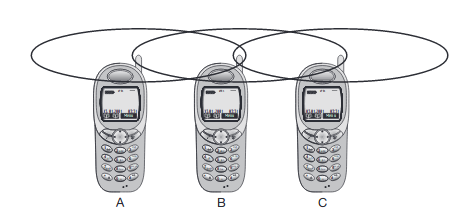
\includegraphics[width=250pt]{hidden_terminal.png}
\end{figure}
\end{document}
